\chapter{Diagrama de componentes}	
	Los diagramas de componentes son herramientas de UML que permiten ilustrar piezas de software, que representar un elemento importante en el desarrollo de un proyecto sin la necesidad de demostrar cual es la funcionalidad que este tiene dentro del mismo, lo cual hace transparente al usuario final, sabe lo qué hace, más no le interesa cómo lo hace. En la siguiente imágen se muestra el esquema de un diagrama de componentes con sus diversos elementos.
	
\begin{figure}[h!]
	\centering
	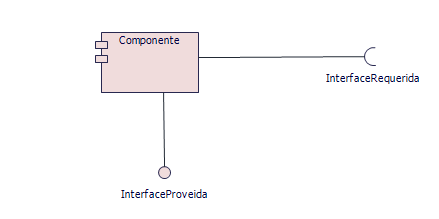
\includegraphics[scale=0.8]{diseno/componentes/imgs/comp}
	\caption{Diagrama Componentes}
\end{figure}

\subsection{ELEMENTOS}
Más allá del esquema de componentes, hay algo muy importante que toca tener en cuenta y son las interfaces. Las interfaces al ser abstracciones puras nos permiten generalizar y abstraer, valga la redundancia, los métodos más importantes que utilizarán los componentes. 

Los componentes se relacionan con dichas interfaces de dos maneras posibles, proveyendolas o requiriendolas.

En caso de que sea una interfaz  proveida estamos hablando de aquellas cosas que el componente es capaz de realizar y que pone a servicio de otros componentes, mientras que si es una interfaz requerida son los elementos que un componente necesita para funcionar.

En la siguiente imagen se muestra el diagrama de componetes propues para el proyecto Cine+.
\begin{figure}[h!]
	\centering
	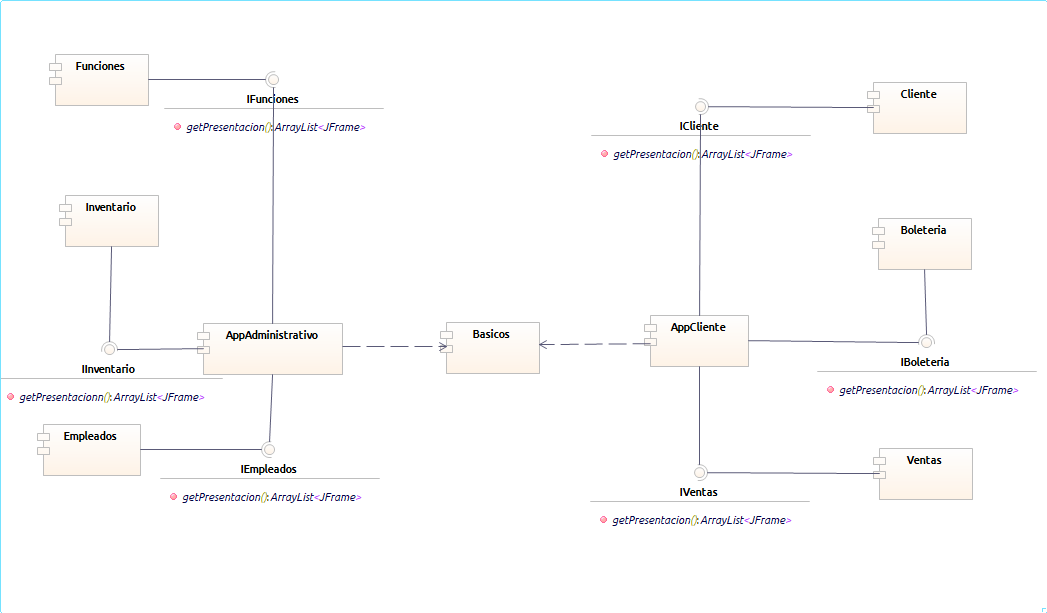
\includegraphics[scale=0.8]{diseno/componentes/imgs/compCine+}
	\caption{Diagrama Componentes de Cine+}
\end{figure}